\section{Additional figure}\label{S1A1}

\subsection{ Outcome for different model order}\label{A1}




\begin{figure}[!htbp]
\foreach \i in {3,...,10} {%
    \begin{subfigure}[p]{0.5\textwidth}
        \includegraphics[width=0.85\linewidth]{\i}
    \end{subfigure}\quad
}
\end{figure}



\begin{figure}[!htbp]
\foreach \i in {11,...,18} {%
    \begin{subfigure}[p]{0.5\textwidth}
        \includegraphics[width=0.85\linewidth]{\i}
    \end{subfigure}\quad
}
\end{figure}


\begin{figure}[!htbp]
\foreach \i in {19,...,26} {%
    \begin{subfigure}[p]{0.5\textwidth}
        \includegraphics[width=0.85\linewidth]{\i}
    \end{subfigure}\quad
}
\end{figure}


\begin{figure}[!htbp]
\foreach \i in {27,...,28} {%
    \begin{subfigure}[p]{0.5\textwidth}
        \includegraphics[width=0.85\linewidth]{\i}
    \end{subfigure}\quad
}
\end{figure}


\begin{figure}[!htbp]
\centering
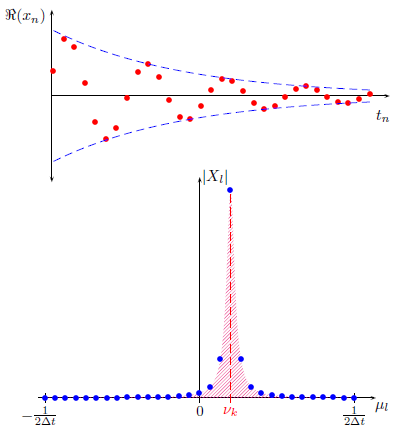
\includegraphics[width=0.5\textwidth]{icon3.png}\\
\caption{Exponentially damping sinusoidal underlying model}\label{EDS}
\end{figure}
